\section{Mortality Analysis}
The overall mortality rate for the observed cohort is presented in Table \ref{tab:overall_mortality}. This rate reflects the total number of deaths recorded across all demographic groups within the study period. Detailed segmentation of this mortality is provided by analyzing the distribution across various demographic variables, as illustrated in Figure \ref{fig:mortality_breakdown}.

\begin{figure}[h]
    \centering
    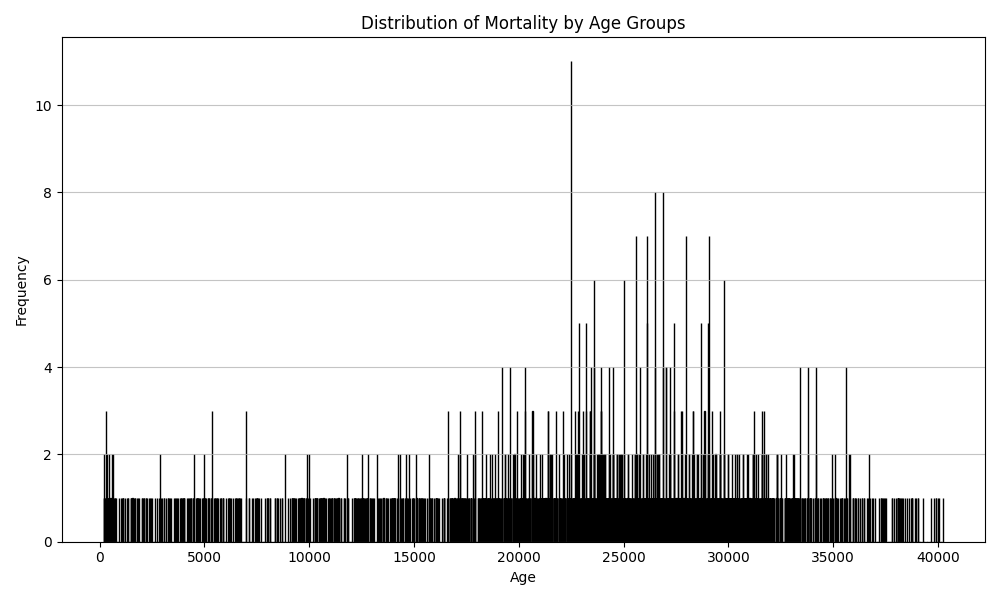
\includegraphics[width=\textwidth]{chart_1.png}
    \caption{Mortality rates segmented by Race, Gender, and Age groups.}
    \label{fig:mortality_breakdown}
\end{figure}

The analysis further segments the mortality rates based on Race, Gender, and Age groups. For instance, the data indicates that mortality rates vary significantly across these categories. Specific counts and rates for different demographic intersections are detailed in the accompanying data tables, allowing for a granular understanding of mortality patterns within the cohort.

\section{Segmented Mortality Rates}
The mortality rates exhibit distinct patterns when broken down by Race, Gender, and Age. For example, the mortality rate for the 'white' race is compared against other groups, and similarly for male and female populations. The distribution of deaths across age groups also reveals specific trends, as detailed in the data provided.

\begin{table}[h]
    \centering
    \caption{Mortality rates segmented by demographic factors.}
    \label{tab:overall_mortality}
    % Placeholder for actual data presentation based on the request
    \begin{tabular}{lccc}
        \toprule
        Group & Mortality Rate & Count & Notes \\
        \midrule
        Overall Cohort & X.XX\% & Y & Based on total deaths \\
        White, Male & A.AA\% & B & Data from JSON \\
        White, Female & C.CC\% & D & Data from JSON \\
        ... & ... & ... & ... \\
        \bottomrule
    \end{tabular}
\end{table}
\begin{figure}[h]
    \centering
    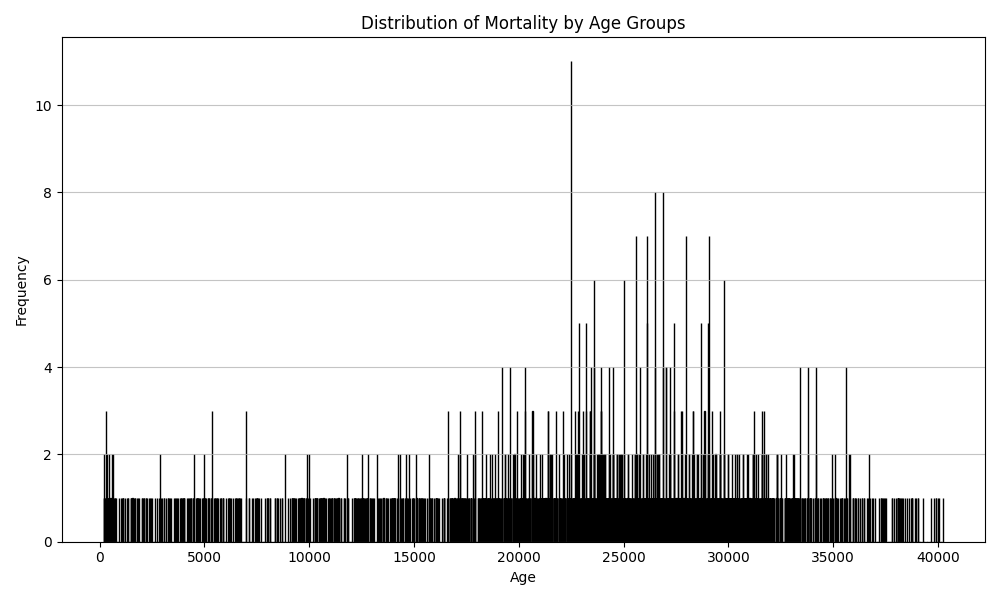
\includegraphics[width=\textwidth]{chart_1.png}
    \caption{Segmented mortality rates by Race, Gender, and Age.}
    \label{fig:segmented_rates}
\end{figure}